\documentclass[a4paper,11pt]{report}
\usepackage{amsmath}
\usepackage{graphicx}
\usepackage{wrapfig}
\usepackage{caption}
\usepackage{enumitem}
\usepackage{pdfpages}
\usepackage{multicol}
\usepackage[a4paper, left=3cm, right=3cm, top=3cm, bottom=3cm]{geometry}
\usepackage[ngerman]{babel}
\usepackage{hyperref}
\usepackage[x11names]{xcolor}
\usepackage{fancyhdr}
\pagestyle{fancy}
\usepackage{tikz}
\usetikzlibrary{calc}
\usepackage{titling}
\usepackage{fontspec}
\usepackage{titlesec}
\usepackage{moresize}
\usepackage{pgfplots}
\pgfplotsset{compat=1.15}

\usepackage{mathrsfs}
\usetikzlibrary{arrows}

% font setup
\newfontfamily{\newUpperTitleFont}{Bebas Neue}
\newfontfamily{\newLowerTitleFont}{Tex Gyre Heros Bold}

% font init
\titleformat{\part}[display]{\centering\HUGE\scshape\newUpperTitleFont\color{SlateBlue4}}{\partname~\thepart}{10pt}{}
\titleformat{\chapter}{\Huge\bfseries\newUpperTitleFont\color{SlateBlue4}}{\thechapter}{1em}{}
\titleformat*{\section}{\Large\bfseries\newLowerTitleFont\color{SlateBlue3}}
\titleformat*{\subsection}{\large\bfseries\newLowerTitleFont\color{SlateBlue2}}

% hyperlink setup
\hypersetup{
    colorlinks,
    citecolor=black,
    filecolor=black,
    linkcolor=SlateBlue3,
    urlcolor=black
}

% clear Footer
\fancyfoot{}

% Header
\fancyhead[L]{Niklas Fister}
\fancyhead[C]{Kantonnschule - Mathematik}
\fancyhead[R]{\thepage}
\renewcommand{\headrulewidth}{1pt}

\fancypagestyle{plain}{
    \fancyhead[L]{Niklas Fister}
    \fancyhead[C]{Kantonnschule - Mathematik}
    \fancyhead[R]{\thepage}
    \renewcommand{\headrulewidth}{1pt}
}

% Title
\title{\Huge\textbf{Bericht Physik - Lautsprecher}}
\author{Niklas Fister}
\date{\today}

% makeing title
\begin{document}
\pagenumbering{Roman}

% pretitle
%
\includepdf[scale=1.05]{resources/pdf/Title.pdf}

% own title
\begin{titlepage}
    \centering
    \begin{tikzpicture}[remember picture, overlay]
        \draw[line width=5pt, line cap=round, color=SlateBlue1, rounded corners=5pt]($(current page.west)+(1cm, 0)$) -- ($(current page.north west)+(1cm, -1cm)$) -- ($(current page.north)+(0, -1cm)$);
        \draw[line width=5pt, line cap=round, color=SlateBlue1, rounded corners=5pt]($(current page.east)+(-1cm, 0)$) -- ($(current page.south east)+(-1cm, 1cm)$) -- ($(current page.south)+(0, 1cm)$);
    \end{tikzpicture}

    % background
    \tikz[remember picture,overlay] \node[opacity=0.3,inner sep=0pt] at (current page.center){
\includegraphics[width=\paperwidth - 4cm, height=\paperheight - 4cm]{resources/images/Mandelbrotmenge.jpg}};
    % Start Text
    \vspace{4cm}

    % the title
    {\newUpperTitleFont\thetitle\par}
    \vspace{1cm}

    % the autors
    {\theauthor\par}
    \vspace{.5cm}

    % date
    {\thedate\par}
    \vspace{5cm}

    % showcase
    %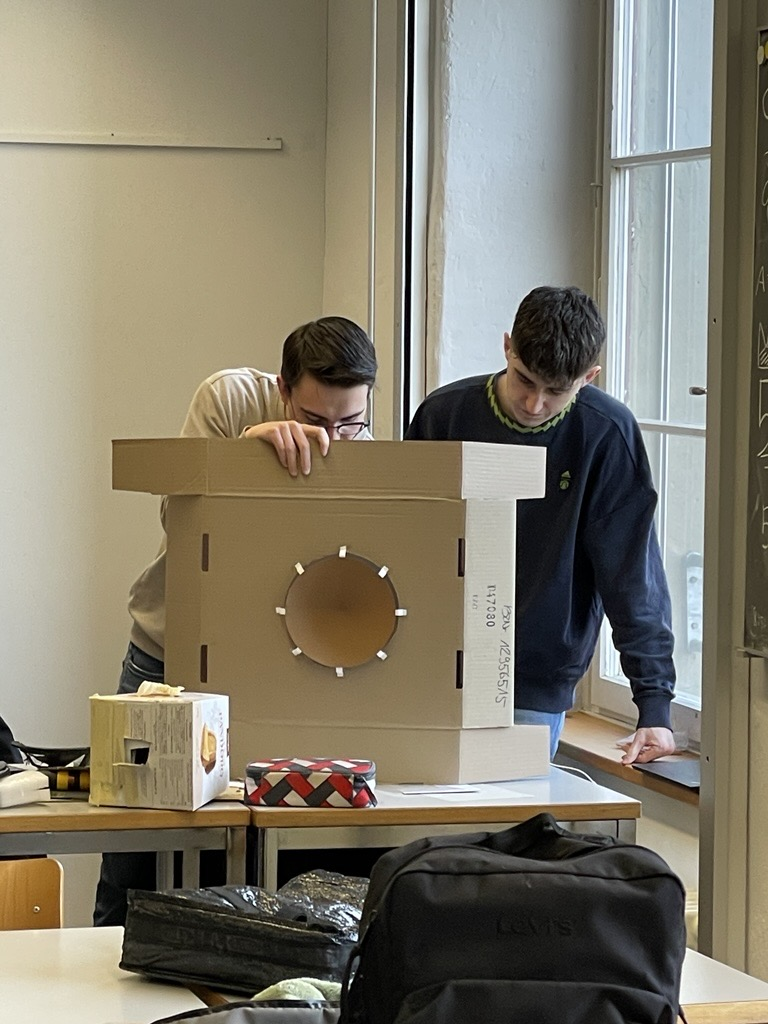
\includegraphics[width=.4\linewidth]{resources/images/Andrin_Cyrill_building.jpeg}
\end{titlepage}
\part{Analysis}
\chapter{Graphischer Zusammenhang der Analysis}
\section{Bedeutung der Ableitung}
Die Ableitung ist die Funktion, welche die Steigung einer anderen Funktion an einem bestimmten Wert für $x$ angibt. 

Es lässt sich somit an dem $y$-Wert der abgeleiteten Funktion die Steigung graphisch, sowie auch numerisch bestimmen.\\

Um dies algebraisch zu bestimmen verwendet man den Limes:
\begin{equation}
    f'(x) = \lim_{h \to 0} \frac{f(x+h) - f(x)}{h}
\end{equation}

Diese Formel ist nichts weiteres als das vorhin erwähnte $\frac{\Delta y}{\Delta x}$, jedoch wurde hier die Funktion eingesetzt.

Man nimmt einen Punkt $x$, sowieso den um $h$ vergrösserten und erhält damit die Formel. Durch den Limes wird der Abstand $h$ 0 angenähert und somit erhält man die Tangente.
\begin{center}
    \begin{tikzpicture}
        \begin{axis}[
            axis lines = middle,
            width=.8\linewidth,
            ymin=-25,ymax=20,
            xmin=-5,xmax=10,
            xlabel=$x$,
            ylabel=$y$,
        ]
        \addplot[smooth, thick, SlateBlue4, domain=-5:10]{x^3 - 3*x^2 - 9*x + 5}; 
        \addplot[smooth, thick, SlateBlue1, domain=-5:10]{3*x^2-6*x-9}; 
        \legend{$f(x) = x^3 - 3\cdot x^2 - 9\cdot x + 5$, $f'(x) = 3\cdot x^2 - 6\cdot x - 9$}
        \end{axis}
    \end{tikzpicture}
\end{center}

\noindent Dies lässt sich in dieser Grafik gut erkennen. Die abgeleitete Funktion $f'(x)$ gibt die Steigung der Funktion $f(x)$ an.

\newpage
\section{Graphische Darstellung des Differential}
Wie man jedoch schrittweise auf die Lösung kommt ist folgendermassen. Hierfür beginnen wir mit einer einfachen Funktion $f(x) = x^2$.
Um die Steigung der Funktion zu bekommen, braucht man eine Tangente zu der Funktion. Die Tangente bekommt man in dem man $\frac{\Delta x}{\Delta y}$ berechnet.

\begin{minipage}{.5\textwidth}
    Es lässt sich an diesem Graphen erkennen, dass die Gerade durch der Tangente annähert, aber noch nicht gleich ist.

    Nun wird man den Abstand verkleinern, bis die Gerade und die Tangente equivalänt sind.
\end{minipage}
\hspace{0.1\textwidth}
\begin{minipage}{.4\textwidth}
    \begin{tikzpicture}[line cap=round,line join=round,>=triangle 45]
        \begin{axis}[
        x=.5cm,y=.5cm,
        axis lines=middle,
        xmin=-5,
        xmax=5,
        ymin=-1,
        ymax=10,
        xtick={-4,-2,...,4},
        ytick={-1,0,5,10},]
        \clip(-5,-1) rectangle (5,10);
        % the functions
        \draw[line width=1pt,smooth,samples=100,domain=-5:5] plot(\x,{(\x)^(2)});
        \draw [line width=1pt,color=SlateBlue1,domain=-5:5] plot(\x,{(-1.2204223944078445--1.9330321397125094*\x)/0.7126097453046649});
        \draw [line width=1pt,color=OrangeRed1,domain=-5:5] plot(\x,{(-1--2*\x)/1});
        % the lines for illustration
        \draw [line width=1pt,color=SeaGreen3, dash pattern=on 1pt off 2pt] (1,1)-- (1.712609745304665,1);
        \draw [line width=1pt,color=SeaGreen3, dash pattern=on 1pt off 2pt] (1.712609745304665,1)-- (1.712609745304665,2.9330321397125094);
        % The two points
        \draw [color=SeaGreen3, fill=SeaGreen3] (1,1) circle (1.5pt);
        \draw [color=SeaGreen3 , fill=SeaGreen3] (1.712609745304665,2.9330321397125094) circle (1.5pt);
        \begin{scriptsize}
        \draw[color=SeaGreen3] (1.6,0.6) node {$\Delta x$};
        \draw[color=SeaGreen3] (2.3,1.8) node {$\Delta y$};
        \draw[color=SeaGreen3] (.5,1.2) node {$A$};
        \draw[color=SeaGreen3] (1.3,3.2) node {$B$};
        \draw[color=black] (1.5,9) node [scale=0.7] {$f(x) = x^2$};
        \draw[color=OrangeRed1] (3.5,4) node [scale=0.5] {$Tangente$};
        \end{scriptsize}
        \end{axis}
    \end{tikzpicture}
\end{minipage}

In einzelnen Etappen darstellt sieht das folgendermassen aus: \\
\begin{minipage}{.5\textwidth}
    \begin{center}
        \begin{tikzpicture}[line cap=round,line join=round,>=triangle 45]
            \begin{axis}[
            x=.5cm,y=.5cm,
            axis lines=middle,
            xmin=-5,
            xmax=5,
            ymin=-1,
            ymax=10,
            xtick={-4,-2,...,4},
            ytick={-1,0,5,10},]
            \clip(-5,-1) rectangle (5,10);
            % the functions
            \draw[line width=1pt,smooth,samples=100,domain=-5:5] plot(\x,{(\x)^(2)});
            \draw [line width=1pt,color=SlateBlue1,domain=-5:5] plot(\x,{(-0.5866610252431241--1.0013527903985366*\x)/0.4146917651554125});
            \draw [line width=1pt,color=OrangeRed1,domain=-5:5] plot(\x,{(-1--2*\x)/1});
            \begin{scriptsize}
                \draw[color=black] (1.5,9) node [scale=0.7] {$f(x) = x^2$};
                \draw[color=OrangeRed1] (3.5,4) node [scale=0.5] {$Tangente$};
            \end{scriptsize}
            \end{axis}
        \end{tikzpicture}
    \end{center}
\end{minipage}
\begin{minipage}{.5\textwidth}
    \begin{center}
        \begin{tikzpicture}[line cap=round,line join=round,>=triangle 45]
            \begin{axis}[
            x=.5cm,y=.5cm,
            axis lines=middle,
            xmin=-5,
            xmax=5,
            ymin=-1,
            ymax=10,
            xtick={-4,-2,...,4},
            ytick={-1,0,5,10},]
            \clip(-5,-1) rectangle (5,10);
            % the functions
            \draw[line width=1pt,smooth,samples=100,domain=-5:5] plot(\x,{(\x)^(2)});
            \draw [line width=1pt,color=SlateBlue1,domain=-5:5] plot(\x,{(-0.26685783030006305--0.4857860814489958*\x)/0.21892825114893277});
            \draw [line width=1pt,color=OrangeRed1,domain=-5:5] plot(\x,{(-1--2*\x)/1});
            \begin{scriptsize}
                \draw[color=black] (1.5,9) node [scale=0.7] {$f(x) = x^2$};
                \draw[color=OrangeRed1] (3.5,4) node [scale=0.5] {$Tangente$};
            \end{scriptsize}
            \end{axis}
        \end{tikzpicture}
    \end{center}
\end{minipage}
\begin{minipage}{.5\textwidth}
    \begin{center}
        \begin{tikzpicture}[line cap=round,line join=round,>=triangle 45]
            \begin{axis}[
            x=.5cm,y=.5cm,
            axis lines=middle,
            xmin=-5,
            xmax=5,
            ymin=-1,
            ymax=10,
            xtick={-4,-2,...,4},
            ytick={-1,0,5,10},]
            \clip(-5,-1) rectangle (5,10);
            % the functions
            \draw[line width=1pt,smooth,samples=100,domain=-5:5] plot(\x,{(\x)^(2)});
            \draw [line width=1pt,color=SlateBlue1,domain=-5:5] plot(\x,{(-0.13280363043648746--0.2515148962434772*\x)/0.11871126580698976});
            \draw [line width=1pt,color=OrangeRed1,domain=-5:5] plot(\x,{(-1--2*\x)/1});
            \begin{scriptsize}
                \draw[color=black] (1.5,9) node [scale=0.7] {$f(x) = x^2$};
                \draw[color=OrangeRed1] (3.5,4) node [scale=0.5] {$Tangente$};
            \end{scriptsize}
            \end{axis}
        \end{tikzpicture}
    \end{center}
\end{minipage}
\begin{minipage}{.5\textwidth}
    \begin{center}
        \begin{tikzpicture}[line cap=round,line join=round,>=triangle 45]
            \begin{axis}[
            x=.5cm,y=.5cm,
            axis lines=middle,
            xmin=-5,
            xmax=5,
            ymin=-1,
            ymax=10,
            xtick={-4,-2,...,4},
            ytick={-1,0,5,10},]
            \clip(-5,-1) rectangle (5,10);
            % the functions
            \draw[line width=1pt,smooth,samples=100,domain=-5:5] plot(\x,{(\x)^(2)});
            \draw [line width=1pt,color=SlateBlue1,domain=-5:5] plot(\x,{(-0.025258746556910072--0.04990981780037007*\x)/0.02465107124346});
            \draw [line width=1pt,color=OrangeRed1,domain=-5:5] plot(\x,{(-1--2*\x)/1});
            \begin{scriptsize}
                \draw[color=black] (1.5,9) node [scale=0.7] {$f(x) = x^2$};
                \draw[color=OrangeRed1] (3.5,4) node [scale=0.5] {$Tangente$};
            \end{scriptsize}
            \end{axis}
        \end{tikzpicture}
    \end{center}
\end{minipage}
Es ist klar eine tendenz zu sehen, dass sich die Geraden immer mehr annähern. Wenn durch den Limes nun dieser Abstand unendlich klein wird, konvergierren diese Geraden und werden zu einer.
\section{Graphische Darstellung des Integral}
\section{Graphischer Zusammenhang der Beiden}
\end{document}